\chapter{Configuring Logging}

\section{Understanding rsyslogd and journald logging}
On RHEL 7 there are two systems responsible for logging : \textbf{rsyslogd} and \textbf{journald}. These two services together to handle logging system information. 

It is up to the services (containing the logging information) to decide how and where the log files will be written to. It is possible to write directly to a log file anywhere (e.g., \verb|/somewhere/my.log|). The service may also choose to pass over the information to \textbf{systemctl} as well. The \verb|systemctl| utility is used to start the service and keep track of the actions of the service while it's starting. Anything that goes through \textbf{systemd} will be writing to \verb|journald|, which is the systemd way of logging. 

\begin{figure}[H]
	\centering
	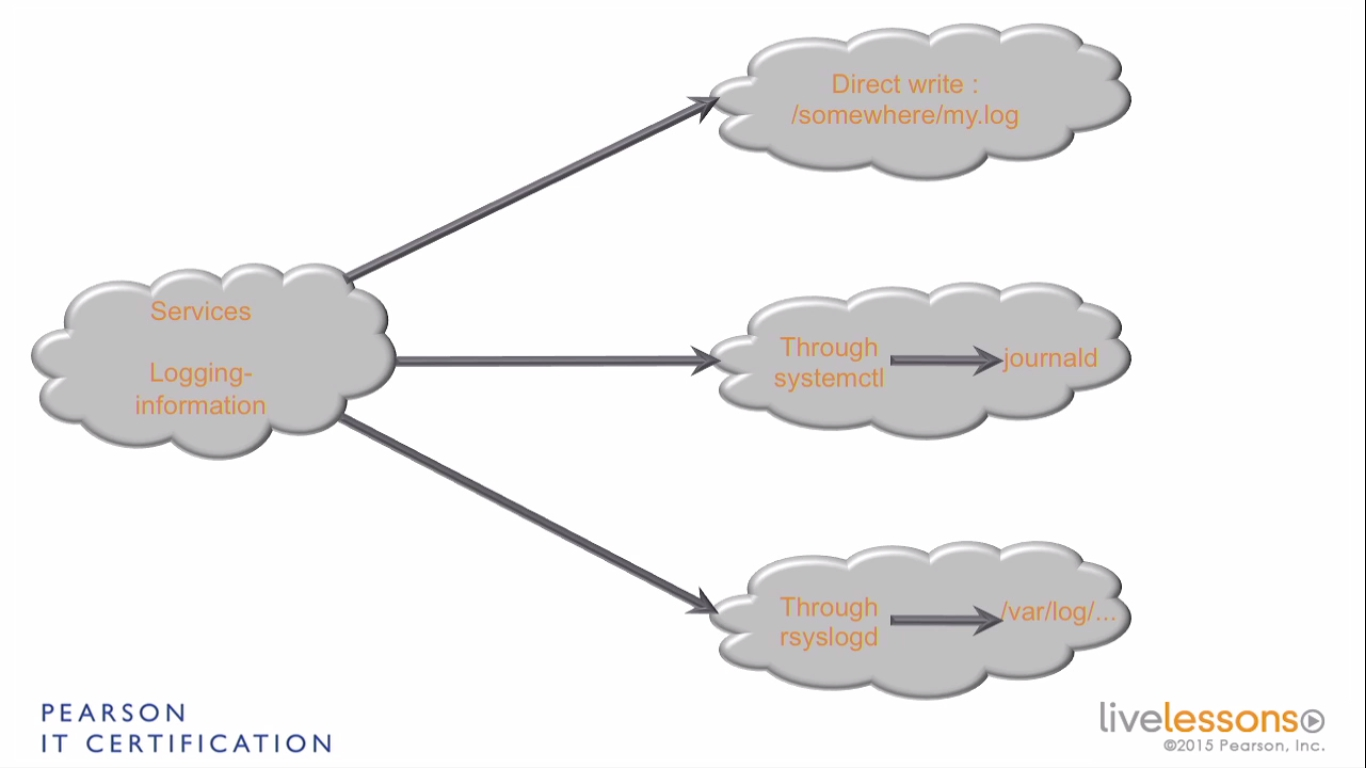
\includegraphics[width=0.9\linewidth]{RHCSA/Mod2/chapters/2.14.a}
	\caption{Logging Options}
	\label{fig:2 Logging Options}
\end{figure}


\noindent
The classic way of logging is through the \verb|rsyslogd| daemon, which typically writes information to the \verb|/var/log/| directory. Alternative locations can also be used. 

Given the various ways to log information, it may also become challenging for a user to get that logged information. It can be through \textbf{journalctl} or rsyslog. It is possible to tie these two systems together.

\subsection{Sharing logging information}	
To ensure that journalctl information is automatically logged to rsyslog, we need to add a couple of lines to \verb|/etc/rsyslog.conf| and \verb|/etc/rsyslog.d/listend.conf|:

\noindent
\begin{tabular}{M{0.47}|M{0.47}}
	\toprule
	In \textbf{/etc/rsyslog.conf} : &In \textbf{/etc/rsyslog.d/listend.conf} : \\
	\midrule
	\begin{minipage}{\linewidth}
		\begin{minted}[frame=none,linenos=none]{bash}
$ModLoad imuxsock
$OmitLocalLogging off
		\end{minted}
		\vspace{-10pt}
	\end{minipage}
	
	&\begin{minipage}{\linewidth}
		\begin{minted}[frame=none,linenos=none]{bash}
$SystemLogSocketName /run/systemd/journal/syslog
		\end{minted}
		\vspace{-10pt}
	\end{minipage}
	\\
	\bottomrule
\end{tabular}

\noindent
The above lines enable rsyslog to receive information logged by journald. To enable the logging of rsyslog information in journald, we only need to add in the \verb|/etc/rsyslog.conf|:

\vspace{-15pt}
\begin{minted}{bash}
$Modload omjournal *.* :omjournal:
\end{minted}
\vspace{-10pt}

\noindent
The above lines specify that any information being logged should be sent to \verb|omjournal| which is a part of journald. The information from there is available from \verb|journalctl|.

\begin{figure}[H]
	\centering
	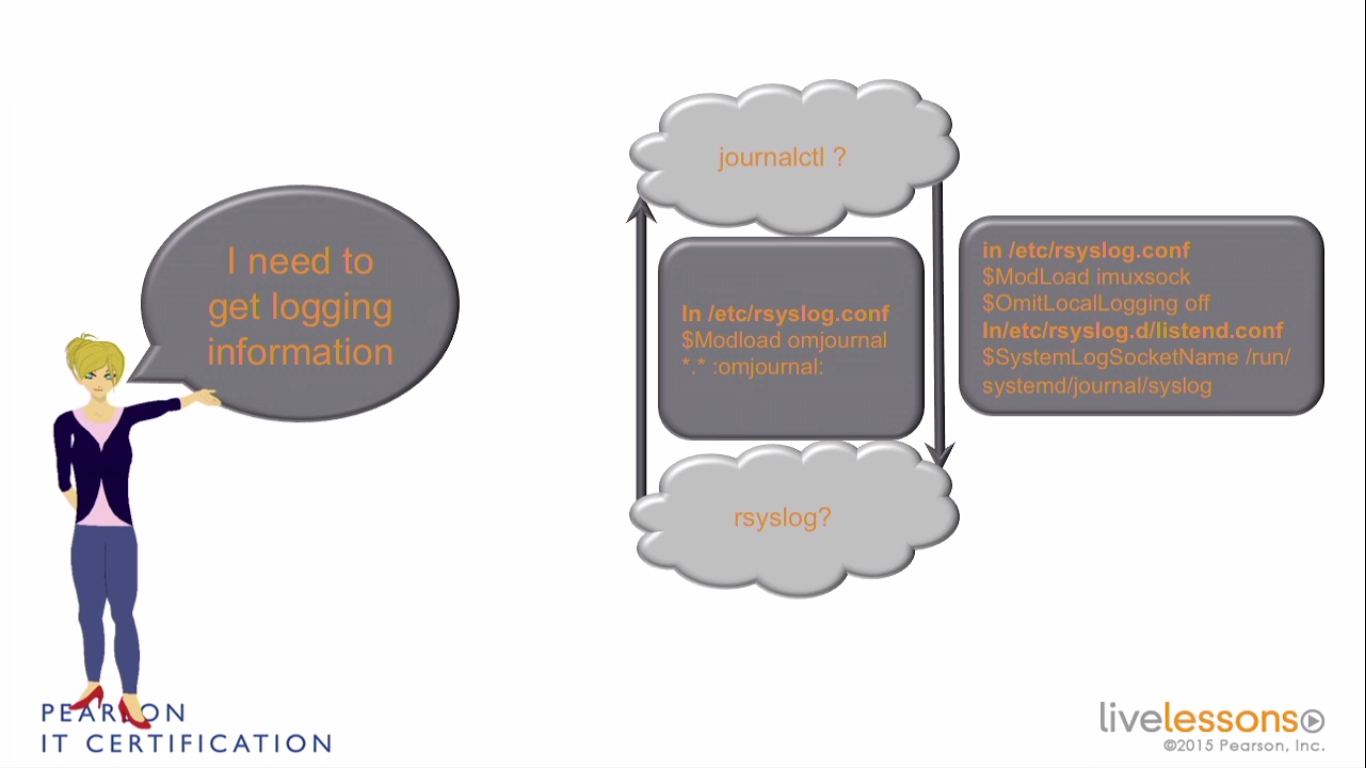
\includegraphics[width=0.9\linewidth]{RHCSA/Mod2/chapters/2.14.b}
	\caption{Sharing logging information between rsyslog and journald}
	\label{fig:2 Sharing logging information}
\end{figure}

	\section{Integrating rsyslogd and journald} 
Rsyslog is the old process of logging system information, and journald is the new process that's trying to do the same. Both of them are built to log process information.

\subsection{rsyslog}
Let us consider a process that's trying to write what it's doing in log files. It has two options: rsyslog and journald. If it writes to rsyslog, the advantage is that rsyslog is the system process that can handle logging for all processes. Some processes, however, just have some internal logging option (direct writes) thus bypassing rsyslog. A well known example of such a process is the \textit{apache web server}. This is a disadvantage as if every process is doing its own logging, it's harder to manage the whole thing in a centralized way. These processes can however, be configured to write to rsyslog anyway! 

\subsection{journald}
Journald is controlled by \textbf{systemd}, which takes care of starting services while booting. Systemd writes its own information to journald, and thus, if something goes wrong while starting a service, the information is available from \textit{journald}. 

For RHEL 7 in general, \textit{journald} generally takes care of loggin the startup information logging while \textit{rsyslog} takes care of logging current activity of processes.

\section{Configuring rsyslog logging}

\begin{center}
	\verb|[VIDEO TUTORIAL MISSING]|
\end{center}
\vspace{-20pt}

\section{Working with journald}
Everything that \textit{journald} is doing is written to a binary file. The file can be explored using two methods: by using \textbf{systemctl} and \textbf{journalctl}. Journald integrates very well with systemctl and thus, systemctl commands can get information from journald and vice versa. Using \verb|systemctl status <serviceName>| gives us the log information that systemctl receives from the journald environment. 

\subsection{journalctl}
The \verb|journalctl| command opens up the binary file that journald is writing to. Since it's a large file, there are several filtering options:

\subsubsection{journalctl -b}
\vspace{-10pt}
The \verb|journal -b| command only shows us the boot log. 

\vspace{-15pt}
\begin{minted}{console}
# journalctl -b
-- Logs begin at Sat 2017-12-02 15:25:40 IST, end at Mon 2017-12-04 13:23:04 IST. --
Dec 02 15:25:40 vmPrime.somuVMnet.com systemd-journal[86]: Runtime journal is using 8.0M (max allowed 289.5M, trying to leave 434.3M free of 2.
Dec 02 15:25:40 vmPrime.somuVMnet.com kernel: Initializing cgroup subsys cpuset
Dec 02 15:25:40 vmPrime.somuVMnet.com kernel: Initializing cgroup subsys cpu
Dec 02 15:25:40 vmPrime.somuVMnet.com kernel: Initializing cgroup subsys cpuacct
Dec 02 15:25:40 vmPrime.somuVMnet.com kernel: Linux version 3.10.0-693.5.2.el7.x86_64 (builder@kbuilder.dev.centos.org) (gcc version 4.8.5 2015
Dec 02 15:25:40 vmPrime.somuVMnet.com kernel: Command line: BOOT_IMAGE=/vmlinuz-3.10.0-693.5.2.el7.x86_64 root=/dev/mapper/centos-root ro crash
Dec 02 15:25:40 vmPrime.somuVMnet.com kernel: Disabled fast string operations
...
\end{minted}
\vspace{-10pt}

\noindent
One of the best features of journald is that systemd initiates it immediately during boot and thus logs about what happens even during the very first stages of RHEL boot is available. 

\subsubsection{journalctl --since=<time>}
\vspace{-10pt}
The journalctl has a method to filter all results to show us what has happened since a specified period where only the logs written after a certain period are show.

\vspace{-15pt}
\begin{minted}{console}
# journalctl --since=yesterday
-- Logs begin at Sat 2017-12-02 15:25:40 IST, end at Mon 2017-12-04 13:28:03 IST. --
Dec 03 23:04:36 vmPrime.somuVMnet.local systemd[1]: Time has been changed
Dec 03 23:04:36 vmPrime.somuVMnet.local NetworkManager[834]: <info>  [1512322476.5889] audit: op="sleep-control" arg="off" pid=3311 uid=0 resul
Dec 03 23:04:36 vmPrime.somuVMnet.local systemd[1]: Stopping LSB: Bring up/down networking...
...
\end{minted}
\vspace{-10pt}

\subsubsection{journald -u}
\vspace{-10pt}
The \verb|journal -u| command shows us all the logs corresponding to a certain process. 

\vspace{-15pt}
\begin{minted}{console}
# systemctl status atd -l
atd.service - Job spooling tools
Loaded: loaded (/usr/lib/systemd/system/atd.service; enabled; vendor preset: enabled)
Active: active (running) since Sat 2017-12-02 15:26:18 IST; 1 day 22h ago
Main PID: 1224 (atd)
CGroup: /system.slice/atd.service
1224 /usr/sbin/atd -f

Dec 02 15:26:18 vmPrime.somuVMnet.local systemd[1]: Started Job spooling tools.
Dec 02 15:26:18 vmPrime.somuVMnet.local systemd[1]: Starting Job spooling tools...
# journalctl -u atd
-- Logs begin at Sat 2017-12-02 15:25:40 IST, end at Mon 2017-12-04 13:37:28 IST. --
Dec 02 15:26:18 vmPrime.somuVMnet.local systemd[1]: Started Job spooling tools.
Dec 02 15:26:18 vmPrime.somuVMnet.local systemd[1]: Starting Job spooling tools...
\end{minted}
\vspace{-10pt}

\noindent
Both systemctl and journald are intimately interconnected. Journald receives it's original logging information from systemctl, while the information displayed by the \verb|systemctl status| command is derived from the information stored by journald. To see the information in even more detail, we use the command \verb|journalctl -u <processName> -o verbose|.

\vspace{-15pt}
\begin{minted}{console}
# journalctl -u atd -o verbose
-- Logs begin at Sat 2017-12-02 15:25:40 IST, end at Mon 2017-12-04 13:44:14 IST. --
Sat 2017-12-02 15:26:18.215379 IST [s=7e5f5839...6e;i=8f2;b=f7106...c3;m=25810b8;t=55f58..dd;x=5e9c...46]
PRIORITY=6
_UID=0
_GID=0
_BOOT_ID=f7106b6e5bc144bcac5827c5089f23c3
_MACHINE_ID=9d29aa554cfa4853b59f2d517a8470bd
SYSLOG_FACILITY=3
SYSLOG_IDENTIFIER=systemd
...
\end{minted}
\vspace{-10pt}

\noindent
The above command gives us complete information about the environment of the process. 

	\section{Understanding logrotate}
Logrotate is a system that's used to ensure that logging doesn't fill the hard disk of the server. Logrotate ensures that after a specified amount of time, log files will be closed and new ones opened, and a backlog of a couple of log files will be kept. This is all done based on the assumption that old logs are useless beyond a certain age. This has a stark disadvantage of erasing logging data that may become useful at a later date. 

A solution to this problem is the use of a log server, with sufficient hard disk space to keep about a year's worth of logs. The client machines can have logrotate setup to keep only a couple of week's data since there will be a backup available on the log server. 

\section{Configuring logrotate}
The configuration files for \verb|logrotate| reside in the \verb|/etc| directory. The generic logrotate configuration is stored in \verb|/etc/logrotate.conf| while the directory \verb|/etc/logrotate.d| contains include files that RPMs dump in it for package specific log rotation. Anything in the \verb|logrotate.d| directory will always overwrite the settings in \verb|logrotate.conf|. Typical contents of the \verb|logrotate.conf| file is:

\vspace{-15pt}
\begin{minted}{bash}
# see "man logrotate" for details
# rotate log files weekly
weekly

# keep 4 weeks worth of backlogs
rotate 4

# create new (empty) log files after rotating old ones
create

# use date as a suffix of the rotated file
dateext

# uncomment this if you want your log files compressed
#compress

# RPM packages drop log rotation information into this directory
include /etc/logrotate.d

# no packages own wtmp and btmp -- we'll rotate them here
/var/log/wtmp {
monthly
create 0664 root utmp
minsize 1M
rotate 1
}

/var/log/btmp {
missingok
monthly
create 0600 root utmp
rotate 1
}
\end{minted}
\vspace{-10pt}

The last two settings demonstrate how specific logrotation instructions can be given for specific files. For example, the \verb|/var/log/wtmp| file has to be rotated monthly, and only 1 copy of the backlog is maintained. 

Since logrotate doesn't need to run all the time, it doesn't itself run as a service, but as a cron job! The config file for  logrotate cron job is \verb|/etc/cron.daily/logrotate|.

\subsection{Checking avialable hard disk space}
The available hard disk space and the disk space occupied by a certain directory can be checked using these two commands:

\vspace{-15pt}
\begin{minted}{console}
# df -h
Filesystem               Size  Used Avail Use% Mounted on
/dev/mapper/centos-root  3.8G  3.4G  412M  90% /
devtmpfs                 2.9G     0  2.9G   0% /dev
tmpfs                    2.9G     0  2.9G   0% /dev/shm
tmpfs                    2.9G  9.2M  2.9G   1% /run
tmpfs                    2.9G     0  2.9G   0% /sys/fs/cgroup
/dev/mapper/centos-home  7.5G   65M  7.4G   1% /home
/dev/mapper/centos-var   1.9G  327M  1.6G  18% /var
/dev/sda2                485M  227M  258M  47% /boot
tmpfs                    580M  4.0K  580M   1% /run/user/42
tmpfs                    580M   28K  580M   1% /run/user/1000
/dev/sr0                 8.1G  8.1G     0 100% /run/media/somu/CentOS 7 x86_64
tmpfs                    580M     0  580M   0% /run/user/0
# du -hs /var/log
13M	/var/log
\end{minted}
\vspace{-10pt}

